\subsection{Temporally Sensitive Pretraining of Video Encoders for Localization Tasks} \label{appendix:tsp-paper}

\subsubsection{Overview}
Most localization methods use video features extracted by models that are trained for Trimmed 
Action Classification (TAC). They're not necessarily suited for Temporal Action Localization 
(TAL), since TAC-pretrained features tend to be temporally insensitive. For example, R(2+1)D, 
I3D and C3D have become the de facto video feature extractors for TAL, Action Proposal and DVC 
tasks; these are trained on TAC. The reasons for most work using TAC trained video encoders 
are (1) many established models exist for TAC and (2) it is impractical to fit untrimmed 
videos in commodity GPUs without drastically downsampling space or time. 
\cite{alwassel2021tsp}. 

\par Alwassel \textit{et al}, in their 2021 paper titled \textit{TSP: Temporally Sensitive 
Pretraining of Video Encoders for Localization Tasks} introduce a supervised pre-training 
paradigm for TAL. This paradigm also considers background clips (which are not as important as 
for TAC) and global video information, to improve temporal sensitivity.

\subsubsection{Contributions and Findings}
\begin{itemize}
\item TSP trains an encoder to explicitly discriminate between foreground and background clips in untrimmed videos
\item Temporally-sensitive features from TSP improves performance for TAL, action proposal and DVC Tasks
\item Consistent performance gains for multiple algorithms, architectures and datasets
\item TAL performance is boosted on short action instances
\end{itemize}

\subsubsection{Pre-training Methodology}
The major goal of TSP is to incorporate temporal sensitivity in video encoders. Hence, this 
pre-training involves training encoders on the task of classifying foreground clips, and 
classifying whether a clip is inside or outside the action. The data used for TSP consists 
of untrimmed videos with temporal annotations. The video encoder is trained end-to-end, from 
raw video input. From an untrimmed video, $X$ is sampled, which has dimensions $3 \times L 
\times W \times H$, where $L$ is the number of frames and $W$ and $H$ are the frame 
dimensions. 3 is the number of channels, i.e., RGB. Since there is a natural imbalance in 
the annotations of foreground and background clips, $X$ is sampled in a way that an equal 
number of clips from each class is chosen. Each $X$ is annotated with two labels:
\begin{itemize}
\item $y^c$: action class label, *if it is from a foreground clip*
\item $y^r$: binary temporal region label, i.e. whether whether the clip is from a 
foreground/action region ($y^r$ = 1) or background/no-action region ($y^r$ = 0) of the video
\end{itemize}

\paragraph{Local and Global Feature Encoding}
The encoder $E$ transforms a clip $X$ to a local $F$-dimensional feature $f$. Global Video 
Feature (GVF) is the max-pooled feature from all local features. For classifying the 
temporal region (foreground or background), combine each local feature f is combined with 
GVF; hence GVF acts as a conditional vector.

\par The video encoders used are ResNet3D and R(2+1)D, while the datasets used are 
ActivityNet v1.3 and THUMOS-14 \cite{thumos-14}. The classification component involves two  
heads:
\begin{itemize}
\item An $F \times C$ fully connected layer for action classification: $f \rightarrow y^c$  (logits vector)
\item A $2F \times 2$ fully connected layer for temporal region label (background \ foreground): $[f, GVF] \rightarrow y^r$
\end{itemize}

\begin{figure}
\centering
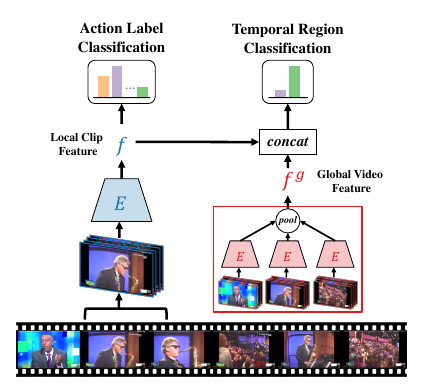
\includegraphics[width=0.5\linewidth]{assets/img/alwassel2021tsp.png}
\caption{The TSP framework. Image courtesy \cite{alwassel2021tsp}}
\label{fig:tsp}
\end{figure}

\par Cross-entropy loss is used for both classification heads. If the clip is a foreground 
clip, then loss from both heads are taken into account, relatively weighted by $\alpha^r$ 
and $\alpha^c$. If the clip is a background clip, only the temporal region classification 
loss is taken, weighted by $\alpha^r$.

\subsubsection{Performance}
Using the pre-trained video encoder, Alwassel \textit{et al} take some implementations of event localisation methods and feed temporally sensitive features to them. The algorithms used are:
\begin{itemize}
\item GTAD: sub-graph localization for Temporal Action Detection
\item BMN: Boundary-matching network for Temporal Action Proposal Generation
\item BMT: Bimodal Transformer for DVC \cite{iashin2020better} (audio features kept same)
\item P-GCN: Graph CNN for Temporal Action Localization
\end{itemize}

Their observations are as follows \cite{alwassel2021tsp}:
\begin{itemize}
\item Improved performance on multiple target tasks, such as TAC, TAL and DVC
\item Consistency of performance regardless of type of video encoder used
\item Consistent improvement in performance for all localization algorithms
\item Indications of applicability of TSP on other datasets as well as its transferability
\end{itemize}

\subsubsection{Conclusion}
Alwassel \textit{et al} present Temporally Sensitive Pretraining, a novel supervised pretraining approach for video encoders. This approach considers background clips along with foreground clips, and uses global information to gain temporal sensitivity. Their results indicate it is advantageous to use TSP features over other popular features to build accurate models \cite{alwassel2021tsp}, especially for DVC.